% Introduction to the prevalent new-user cohort design 
% (c) 2021-2024 Malcolm Gillies <malcolm.gillies@unsw.edu.au>
% https://github.com/mbg-unsw/pnuc
%
% This work is licensed under a
% Creative Commons Attribution-NonCommercial-ShareAlike 4.0
% International Licence
\documentclass[aspectratio=169,12pt]{beamer} % XXXX fix AR here
\usepackage[latin1]{inputenc}
\usepackage[T1]{fontenc}
\usepackage{textcomp}
\usefonttheme{serif} % need this with Charter font
\usetheme{Berlin}  % using default now
\usecolortheme{beaver}  % using default now
\usepackage[libertine]{libertine} % not using osf (old-style figures)
\usepackage[scale=0.9]{tgheros} % scale to match libertine
\usepackage[varqu,varl]{inconsolata}
\usepackage[libertine]{newtxmath}
\usepackage{graphicx}
\usepackage{tikz}
\usetikzlibrary{shadows}
\usepackage{tikzpagenodes}
\usepackage[round]{natbib}
\usepackage{gitinfo2}

\renewcommand{\gitMark}{\color{gray}\texttt{\tiny\gitBranch\,@\,\gitAbbrevHash\,\gitAuthorDate}}

\renewcommand{\bibsection}{} % suppress "References" section

\setbeamertemplate{navigation symbols}{} % remove navigation symbols
\setbeamercolor*{item}{fg=darkred}

\title{UNSW CRAIC: Prevalent new-user cohort design}
\author{Malcolm Gillies}
\institute{\url{https://github.com/mbg-unsw/pnuc}}
\date{5 February 2024}
\usebackgroundtemplate{%
\begin{tikzpicture}[remember picture,overlay]
    \node[anchor=south west,scale=1,rotate=90] at ([shift={(0cm,0cm)}]current page marginpar area.south east) {\gitMark};
\end{tikzpicture}%
}

\newif\ifsidebartheme
\sidebarthemefalse

\newdimen\contentheight
\newdimen\contentwidth
\newdimen\contentleft
\newdimen\contentbottom
\makeatletter
\newcommand*{\calculatespace}{%
    \contentheight=\paperheight%
    \ifx\beamer@frametitle\@empty%
        \setbox\@tempboxa=\box\voidb@x%
      \else%
        \setbox\@tempboxa=\vbox{%
          \vbox{}%
          {\parskip0pt\usebeamertemplate***{frametitle}}%
        }%
        \ifsidebartheme%
          \advance\contentheight by-1em%
        \fi%
      \fi%
    \advance\contentheight by-\ht\@tempboxa%
    \advance\contentheight by-\dp\@tempboxa%
    \advance\contentheight by-\beamer@frametopskip%
    \ifbeamer@plainframe%
    \contentbottom=0pt%
    \else%
    \advance\contentheight by-\headheight%
    \advance\contentheight by\headdp%
    \advance\contentheight by-\footheight%
    \advance\contentheight by4pt%
    \contentbottom=\footheight%
    \advance\contentbottom by-4pt%
    \fi%
    \contentwidth=\paperwidth%
    \ifbeamer@plainframe%
    \contentleft=0pt%
    \else%
    \advance\contentwidth by-\beamer@rightsidebar%
    \advance\contentwidth by-\beamer@leftsidebar\relax%
    \contentleft=\beamer@leftsidebar%
    \fi%
}
\makeatother

\begin{document}

{
%\usebackgroundtemplate{}
\begin{frame}
\titlepage
\end{frame}
}

\begin{frame}{Talk outline}
    \begin{itemize}
	\item Paper background
	\item Prevalent new-user cohort method in detail
	\item Adjusting for informative censoring
	\item Results
	\item What does the PNUC method estimate?
	\item Loose ends
    \end{itemize}
\end{frame}

\begin{frame}{Why \emph{prevalent} new-user?}
    \begin{itemize}
	\item \emph{i.e.} Compare those staying on old tx with switchers to new
	\item Increase sample size if few treatment-naive patients
	\item Better external validity e.g. disease progression
	\item Key feature: conditioning on length of exposure
    \end{itemize}
\end{frame}

\begin{frame}{Review: Active comparator new-user (ACNU) cohort design}
    \begin{itemize}
	\item Problems avoided by the ACNU design
	\begin{itemize}
		\item Confounding by indication (inactive comparator)
		\item Healthy adherer bias (prevalent users)
	\end{itemize}
    \end{itemize}
\end{frame}

\begin{frame}{Popularity of the PNUC design}
% search date
% number of studies
% code not published
% 80% with Suissa's mob
\flushright{\small{\citet{tazare_prevalent_2022}}}
\end{frame}

\begin{frame}{PNUC design in context}
	\centering
	\begin{tabular}{ll}
	\hline
		\bf{No-use} & \bf{Traditional no use} \\
		& \bf{No use episodes} \\
	\hline
		\bf{Active-comparator}  & \bf{Generalized prevalent new user} \\
		& \emph{\bf{Prevalent new user}} \\
		& \bf{Hierarchical prevalent new user} \\
		& \bf{Active comparator new user} \\
	\hline
	\end{tabular}
\flushright{\small{\citet{wintzell_selection_2022}}}
\end{frame}

\begin{frame}{Prevalent new-user cohort design step by step}
    \begin{enumerate}
	\item Defining the base cohort
	\item Forming exposure sets
	\item Estimating the propensity score
	\item Matching and forming the analysis cohort
	\item Estimating the causal effect
    \end{enumerate}
\end{frame}

\begin{frame}{Defining exposure sets and estimating the propensity score}
    \calculatespace%
    \begin{center}
	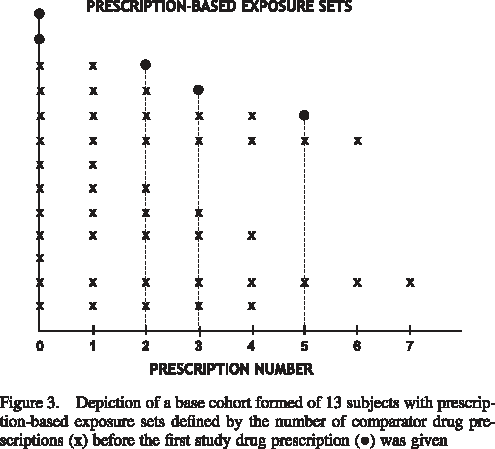
\includegraphics[height=0.85\contentheight]{ref/suimoodell-fig3.pdf}
    \end{center}
\flushright{\small{\citet{suissa_prevalent_2017}}}

\end{frame}

\begin{frame}{Matching}
    \calculatespace%
    \begin{center}
	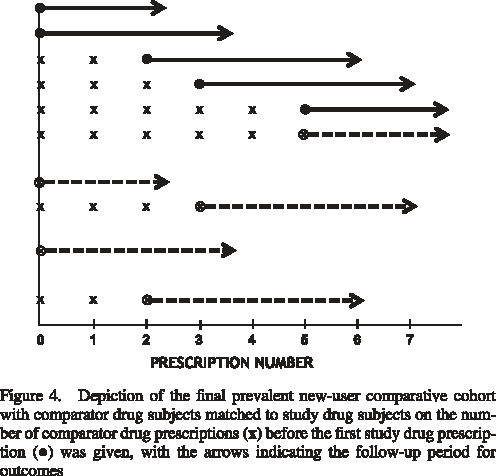
\includegraphics[height=0.85\contentheight]{ref/suimoodell-fig4.pdf}
    \end{center}
\flushright{\small{\citet{suissa_prevalent_2017}}}
\end{frame}

\begin{frame}{Informative censoring among comparator group}
    \begin{itemize}
	\item Follow-up of comparator group is censored if study treatment starts
	\item Starting treatment = patient is still alive (but sicker?)
	\item Remove bias through inverse probability of censoring weights (IPCW)
    \end{itemize}
\end{frame}

\begin{frame}{Example study}
\calculatespace%
\begin{columns}
\begin{column}{0.20\contentwidth}
\begin{tikzpicture}
  \node[drop shadow={shadow xshift=.8ex,shadow yshift=-.8ex},fill=white,draw] at (0,0) {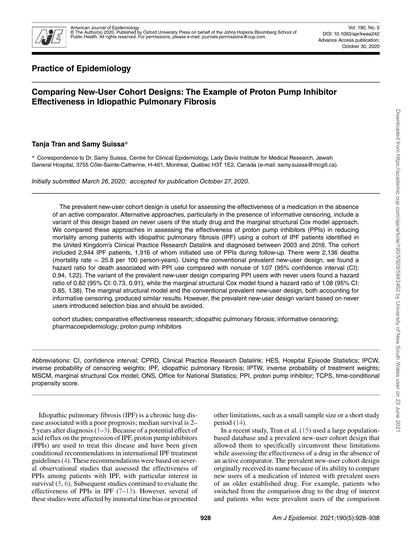
\includegraphics[width=\textwidth]{ref/suissa-pages-01_sm.jpg}};
\end{tikzpicture}
\end{column}
\begin{column}{0.70\contentwidth}
	\begin{itemize}
		\item T.~Tran and S.~Suissa. \textbf{Comparing {New}-{User} {Cohort} {Designs}: {The} {Example} of {Proton} {Pump} {Inhibitor} {Effectiveness} in {Idiopathic} {Pulmonary} {Fibrosis}.} \emph{American Journal of Epidemiology}, 190\penalty0 (5):\penalty0 928--938, May 2021. doi:10.1093/aje/kwaa242.
\nocite{tran_comparing_2021}
	\end{itemize}
\end{column}
\end{columns}
\end{frame}

\begin{frame}{What is the paper about?}
    \begin{itemize}
	\item Question: Are PPIs efficacious in idiopathic pulmonary fibrosis?
	\item Data: UK linked GP and hospital data (CPRD-GOLD/HES/ONS), $n=2944$
	\item Outcomes: All-cause mortality, respiratory death, hospitalisation
	\item Covariates: Demographics, comorbidity, medicines (all time-varying)
	\item Compare results from three different study designs
    \end{itemize}
\end{frame}

\begin{frame}{Idiopathic Pulmonary Fibrosis (IPF)}
    \begin{itemize}
        \item Progressive scarring of the lungs, cause unknown
	\item Average life expectancy after diagnosis about four years
	\item Pirfenidone (2008) and nintedanib (2014) slow progression
	\item Proton pump inhibitors also guideline recommended (weak evidence)
	\item Contention: PPI effects seen in earlier studies are due to bias
    \end{itemize}
\end{frame}

\begin{frame}{Estimands}
    \calculatespace%
    \begin{center}
	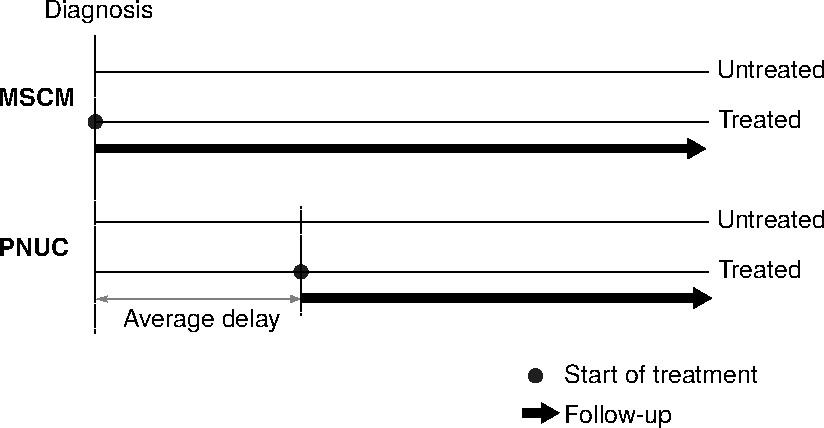
\includegraphics[height=0.95\contentheight]{ref/estimands.pdf}
    \end{center}
\end{frame}

\begin{frame}{Results}
    \calculatespace%
    \begin{center}
	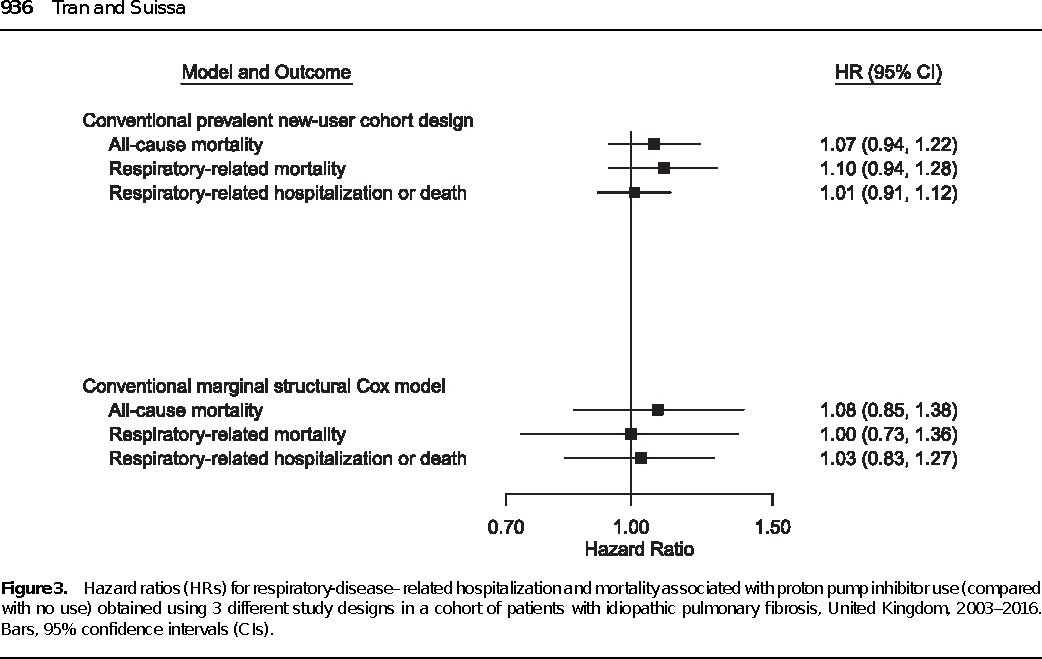
\includegraphics[height=0.90\contentheight]{ref/suissa-fig3-mscm.pdf}
    \end{center}
\end{frame}

\begin{frame}{PNUC vs MSCM}
	\centering
	\begin{tabular}{lll}
	\hline
		& PNUC & MSCM \\
	\hline
		Complexity & XX & XX \\
		Computation & XX & XX \\
		Precision & XX & XX \\
		Estimand & XX & XX \\
	\hline
	\end{tabular}
\flushright{\small{\citet{webster-clark_alternative_2022}}}
\end{frame}

\begin{frame}{PNUC sub-cohorts}
    \calculatespace%
	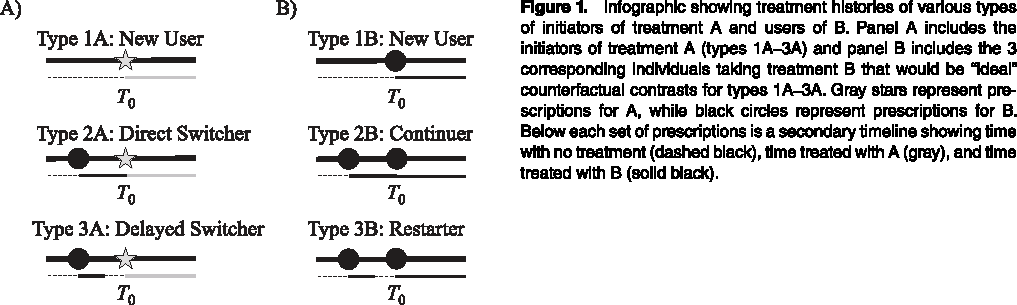
\includegraphics[width=0.85\contentwidth]{ref/webster-fig1.pdf}
\flushright{\small{\citet{webster-clark_initiator_2020}}}
\end{frame}

\begin{frame}{Developments}
    \begin{itemize}
	\item Matching with/without replacement or weighting
	\item How to condition on ``length of exposure''?
	\item Positivity and matching
	\item Estimating the propensity score
    \end{itemize}
\flushright{\small{\citet{webster-clark_presentation_2020}}}
\end{frame}

\begin{frame}{Discussion}
    \begin{itemize}
	\item Have you used the prevalent new-user cohort design or the marginal structural Cox model approach? If so, please tell us about it.
    	\item Would you use either of these methods for your current research interests? What do you see as the barriers to using them?
    \end{itemize}
\end{frame}

\begin{frame}{References}
        \tiny\bibliography{pnuc.bib}
        \bibliographystyle{abbrvnat}
\end{frame}

\begin{frame}{Acknowledgments}
    \begin{itemize}
	\item An earlier version was presented to the Medicine
	Intelligence CRE Methods journal club on 1 July 2021
    \end{itemize}
\end{frame}

\end{document}
